\documentclass[utf8,t,aspectratio=169]{beamer}
\usepackage[ngerman]{babel}
\usepackage{graphicx}
\usepackage{tabularx}
\usepackage{caption}
\usepackage{fontspec}
\usepackage{tikz}
\usepackage[simplified]{pgf-umlcd}
\usetikzlibrary{arrows.meta}
%\usetikzlibrary{positioning}
\usetikzlibrary{calc}
\usetikzlibrary{shapes.geometric}
\usetikzlibrary{shapes.callouts}
\usetikzlibrary{decorations.pathreplacing}

\usepackage{listings}
\definecolor{backcolor}{rgb}{0.95,0.95,0.92}
\lstdefinestyle{standardStyle}{
  language=Java,
	keywordstyle=\bfseries\color{blue},
	numbers=none,
	numbersep=5pt,
	stringstyle=\color{red},
	tabsize=2,
	numberstyle=\small,
	showstringspaces=false,
	basicstyle=\ttfamily,
	breaklines=true,
	backgroundcolor=\color{backcolor},
	breakatwhitespace=false,
	captionpos=b,
  morekeywords={@Test, @DisplayName, @Tag, @RepeatedTest, @BeforEach,
  @AfterEach, @TestTemplate, @ExtendWith, @ParameterizedTest,
  @ValueSource, @Execution, @ResourceLock}
}
\lstset{style=standardStyle}


\graphicspath{{./images/}}

\usetheme{CambridgeUS}
\subtitle{\Large Softwarequalität in der komponentenbasierten Entwicklung}
\title{Modultests mit JUnit}
\author{Simon Döring \and Michael Edelmann}
\date{\today}

\setbeamercovered{transparent}
\beamertemplatenavigationsymbolsempty 
\begin{document}
	\titlegraphic {
		\begin{tikzpicture}[overlay,remember picture]
			\node[left=0.4cm, below=0.3cm, behind path] at (current page.30) {
                \includegraphics[scale=0.4]{logo-hochschule-bochum-bo.pdf}};
			\node[left=2.1cm, below=0.3cm] at (current page.30)
        {\includegraphics[scale=0.4]{logo-hochschule-bochum-text.pdf}};
		\end{tikzpicture}
	}
	\frame{\maketitle}

	\begin{frame}{Agenda}
		\tableofcontents
	\end{frame}

  \section{Einleitung}
    \begin{frame}[fragile]{Wiederholung: Unit-Tests vs. Integrationstests}
      \begin{itemize}
        \item Unit-Tests
          \begin{itemize}
            \item Isoliertes Testen einzelner Klassen und Methoden
            \item Kann Fehler einfach und präsize aufdecken
            \item Beispiel: \glqq{}Funktioniert die Komponente für sich?\grqq
          \end{itemize}
        \item Integrationstests
          \begin{itemize}
            \item Testen des Zusammenspiels mehrerer Softwarebausteine
            \item Kann das Big-Picture der Applikation besser validieren
            \item Beispiel: \glqq{}Funktioniert das Zusammenspiel der Komponenten?\grqq
          \end{itemize}
      \end{itemize}
    \end{frame}
    \begin{frame}[fragile]{Äquivalenzklassentests}
      \begin{itemize}
        \item Annahme: Zu testende Funktionalität verhält sich für bestimmte Klasse von Werten gleich
        \item Tests müssen dann nur für wenige Stichproben aus dieser Äquivalenzklasse ausgeführt werden
        \item Beispiel: Monat
          \begin{itemize}
            \item Werte zwischen 0 bis 11 gültig
            \item Alle anderen Werte ungültig
            \item Beispielhaft zu testende Werte: -5, -1, 0, 5, 11, 12, 17
          \end{itemize}
      \end{itemize}
    \end{frame}
    \begin{frame}{JUnit}
      \begin{itemize}
        \item Testing-Framework für Java und JVM
        \item Release der fünften Version 2017
        \item Einfache und intuitive Verwendung
        \item Ausgereift und viele fortgeschrittene Features
      \end{itemize}
    \end{frame}
  \section{JUnit 5 in Eclipse}
    \begin{frame}[fragile]{Hinweise für die Verwendung von JUnit 5 in Eclipse}
      \begin{itemize}
        \item In den Properties des Projekts muss JUnit 5 dem \textbf{Modulepath} hinzugefügt werden
          \begin{itemize}
            \item Dafür in den Projekt-Properties nach \glqq{}Java Build Path\grqq{} navigieren, dann oben auf \glqq{}Libraries\grqq{} klicken, in der Liste auf \glqq{}Modulepath\grqq{} klicken und JUnit rechts über \glqq{}Add Library\grqq{} hinzufügen
            \item Eclipse fügt JUnit standardmäßig dem \textbf{Classpath} hinzu
          \end{itemize}
        \item In module-info.java zwischen den geschweiften Klammern die Zeile \lstinline{requires org.junit.jupiter.api;} hinzufügen
        \item Ausführen von Tests: Run $\rightarrow$ Run As $\rightarrow$ JUnit Test
      \end{itemize}
    \end{frame}
	\section{Live-Demo}
    \begin{frame}[c]
      \Huge
      \centering
      Live-Demo
    \end{frame}
    \begin{frame}[fragile]{BooleanSupplier und Supplier<String>}
      \begin{itemize}
        \item Functional Interfaces die jeweils \lstinline{boolean} und \lstinline{String} liefern
          \begin{itemize}
            \item Kurzschreibweise durch Lambda-Ausdruck
          \end{itemize}
        \item \lstinline{BooleanSupplier} kann in JUnit-Assertions statt \lstinline{boolean} verwendet werden
        \item \lstinline{Supplier<String>} kann in JUnit-Assertions für Fehlermeldungen verwendet werden
          \begin{itemize}
            \item Verwendung wenn Fehlernachricht nur im Fehlerfall erstellt werden kann
          \end{itemize}
      \end{itemize}
    \end{frame}
    \begin{frame}[fragile]{Anwendungsbeispiel Supplier<String>}
      \begin{lstlisting}[gobble=8]
        import java.util.HashMap; import java.util.function.Supplier;
        import org.junit.jupiter.api.Test;
        import org.junit.jupiter.api.Assertions.*;

        class HashMapTest {
          @Test
          void testLeeresGet() {
            HashMap<String, String> map = new HashMap<>();
            String str = map.get("nicht-existenter schlüssel");
            Supplier<String> fehlerSupplier =
              () -> String.format("'%s' gefunden", str);
            assertNull(str, fehlerSupplier);
          }
        }
      \end{lstlisting}
    \end{frame}
    \begin{frame}[fragile]{Exception Testing mit assertThrows}
      \begin{itemize}
        \item Testen ob bestimmte Benutzung korrekt Exceptions wirft
      \end{itemize}
      \begin{lstlisting}[gobble=8]
        import org.junit.jupiter.api.Test;
        import org.junit.jupiter.api.Assertions.*;

        class ArrayTest {
          @Test
          void testOutOfBoundsIndexing() {
            int[] arr = new int[3];
            assertThrows(IndexOutOfBoundsException.class,
              () -> { int num = arr[5]; });
          }
        }
      \end{lstlisting}
    \end{frame}

  \section{Verschiedene Aspekte von JUnit}
    \begin{frame}[fragile]{DisplayName}
      \begin{itemize}
        \item Spezielle Bezeichnung für Test-Klassen und -Methoden
        \item Ohne Namenskonvention
        \item Anzeige im Testbericht oder in IDEs
      \end{itemize}
      \begin{lstlisting}[gobble=8]
        import org.junit.jupiter.api.DisplayName;
        import org.junit.jupiter.api.Test;

        @DisplayName("Ein spezieller Testfall")
        class DisplayNameTest {

          @Test
          @DisplayName("Eigener Testname, der Leerzeichen enthält")
          void testMitDisplayNameDerLeerzeichenEnthählt() { }
        }
      \end{lstlisting}
    \end{frame}
    \begin{frame}[fragile]{Assertions}
      \begin{itemize}
        \item Annahmen, die Erfolg oder Misserfolg bestimmen
          \item Ergebnis einer Methode, wird mit einem erwarteten Wert
            verglichen
      \end{itemize}
      \begin{lstlisting}[gobble=8]
        import static org.junit.jupiter.api.Assertions.assertEquals;
        import static org.junit.jupiter.api.Assertions.assertNotNull;
        @Test
        void testAssertions() {
          assertEquals(2, 1+1);
          assertNotNull(new Object());
        }
      \end{lstlisting}
    \end{frame}
    \begin{frame}[fragile]{Timeout}
      \begin{itemize}
        \item Durchführung innerhalb einer festen Zeitspanne
      \end{itemize}
      \begin{lstlisting}[gobble=8]
        import static java.time.Duration.ofMinutes;
        import static org.junit.jupiter.api.Assertions.assertTimeout;
        @Test
        void testTimout() {
          assertTimeout(ofMinutes(2), () -> {
            // Lambda-Ausdruck mit Ausgabe, die innerhalb
            // von 2 Minuten ausgeführt werden soll
          }
        }
      \end{lstlisting}
    \end{frame}
    \begin{frame}[fragile]{Assumption}
      \begin{itemize}
        \item Entscheidet, ob ein Test überhaupt ausgeführt werden soll
        \item JUnit Jupiter (JUnit 5) enthält zusätzliche Assumption-Methoden
      \end{itemize}
      \begin{lstlisting}[gobble=8]
        import static org.junit.jupiter.api.Assumptions.assumeTrue;
        @Test
        void testNurAufCIServer() {
          assumeTrue("CI".equals(System.getenv("ENV")));
          // Rest des Tests
        }
        @Test
        void testNurAufEntwicklungsUmgebungen() {
          assumeTrue("DEV".equals(System.getenv("ENV")),
            () -> "Test abbrechen: keine Entwicklungs-Umgebung");
          // Rest des Tests
        }
      \end{lstlisting}
    \end{frame}
    \begin{frame}{Dependency Injection}
      \begin{itemize}
        \item Test-Methoden und -Konstruktoren können Parameter haben
        \item \lstinline|ParameterResolver|: API für Test-Erweiterungen,\\
          mit dynamischer Parameterauflösung zur Laufzeit
        \item Vordefinierte Resolver, die direkt verwendet werden können
          \begin{itemize}
            \item \lstinline|TestInfoParamterResolver|
                \begin{itemize}
                  \item Parameter-Typ \lstinline|TestInfo|
                \end{itemize}
              \item \lstinline|RepetitionInfoParameterResolver|
                \begin{itemize}
                  \item Parameter-Typ \lstinline|RepetitionInfo| in
                    \lstinline|@RepeatedTest|, \lstinline|@BeforEach|,
                    \lstinline|@AfterEach|
                  \item Enthält Informationen über die aktuellen Wiederholung\\
                    und die Gesamtzahl eines sich wiederholenden Test (Repeated
                    Test)
                \end{itemize}
              \item \lstinline|TestReporterParameterResolver|
                \begin{itemize}
                  \item Parameter-Typ \lstinline|TestReporter|
                \end{itemize}
          \end{itemize}
      \end{itemize}
    \end{frame}
    \begin{frame}[fragile]{Dependency Injection}{\lstinline|TestInfo|}
      \begin{itemize}
          \item Instanz entspricht dem aktuellen Container oder Test
          \item Enthält Informationen wie den Display Namen,\\
            die Klasse, Methode und hinzugefügte Tags
      \end{itemize}
      \begin{lstlisting}[gobble=8]
        import org.junit.jupiter.api.TestInfo;
        import org.junit.jupiter.api.Tag;

        @Test
        @DisplayName("TEST 1")
        @Tag("my-Tag")
        void test1(TestInfo testInfo) {
          assertEquals("TEST 1", testInfo.getDisplayName());
          assertTrue(testInfo.getTags().contains("my-tag"));
        }
      \end{lstlisting}
    \end{frame}
    \begin{frame}[fragile]{Dependency Injection}{\lstinline|TestReporter|}
      \begin{itemize}
          \item Zusätzliche Informationen für Test-Berichte über den
            aktuellen Durchlauf
      \end{itemize}
      \begin{lstlisting}[gobble=8]
        import org.junit.jupiter.api.TestReporter;

        @Test
        void reportValue(TestReporter testReporter) {
          testReporter.publishEntry("eine Statusmeldung");
          testReporter.publishEntry("ein Schlüssel", "ein Wert");
          Map<String, String> werte = new HashMap<>();
          values.put("Benutzername", "benutzername");
          values.put("Geburtsjahr", "1974");
          testReporter.publishEntry(werte);
        }
      \end{lstlisting}
    \end{frame}
    \begin{frame}[fragile]{Repeated Tests}
      \begin{itemize}
        \item Test wird komplett eine definierte Anzahl wiederholt
        \item Kompletter Test-Lebenszyklus (\lstinline|@BeforEach|,
          \lstinline|@Test|, \lstinline|@AfterEach|)
        \item Wie wiederholte Definition von \lstinline|@Test|
      \end{itemize}
      \begin{lstlisting}[gobble=8]
        @RepeatedTest(10) 
        void wiederholenderTest() {
          // führt wiederholenderTest 10 Mal aus
        }
      \end{lstlisting}
    \end{frame}

    \begin{frame}[fragile]{Parametrisierte Tests}
      \begin{itemize}
        \item Test mehrfach mit verschiedenen Werten ausführen
        \item Notation mit \lstinline|@ParameterizedTest| anstatt
          \lstinline|@Test|
        \item Erfordert mindestens eine \textit{source} mit Werten für jeden
          Durchlauf
      \end{itemize}
      \begin{lstlisting}[gobble=8]
        @ParameterizedTest
        @ValueSource(strings = {"bob", "radar"})
        void palindromes(String kandidat) {
          assertTrue(StringUtils.isPalindrome(kandidat));
        }
      \end{lstlisting}
    \end{frame}
    \begin{frame}[fragile]{Test-Templates}
      \begin{itemize}
        \item Kein regulärer Testfall, eher eine Vorlage für Testfälle
        \item Mehrfacher Aufruf, durch einen registrierten Anbieter, wie ein
          normaler \lstinline|@Test|
        \item Verbindung mit der
          \lstinline|TestTemplateInvocationContextProvider|
        \item Repeated Test und Parametrisierte Tests sind spezielle
          Test-Templates
      \end{itemize}
    \end{frame}

    \begin{frame}[fragile]{Paralleles Testen}
      \begin{itemize}
        \item Experimentelle Funktion seit JUnit 5.3
        \item \lstinline[keywordstyle=\texttt]|junit.jupiter.execution.parallel.enabled = true|
        \item \lstinline[keywordstyle=\texttt]|junit.jupiter.execution.parallel.mode = concurrent|
        \item \lstinline[keywordstyle=\texttt]|junit.jupiter.execution.parallel.classes.default = concurrent|
        \item Concurrent-Mode auch über Annotation einstellbar
        \item Thread-Sicherheit über \lstinline|@ResourceLock|
      \end{itemize}
      \begin{lstlisting}[gobble=8]
        @Execution(CONCURRENT)
        class GeteilteRessourceTest {
          @Test
          @ResourceLock(value = SYSTEM_PROPERTIES, mode = READ) 
          void getGeteilteRessource() {
            assertNull(System.getProperty("null"));
          }
      \end{lstlisting}
    \end{frame}
    \begin{frame}[c]{Parallele Test-Modi}
      \centering
      \begin{picture}(\textwidth, \textheight)
        \put(40,29){{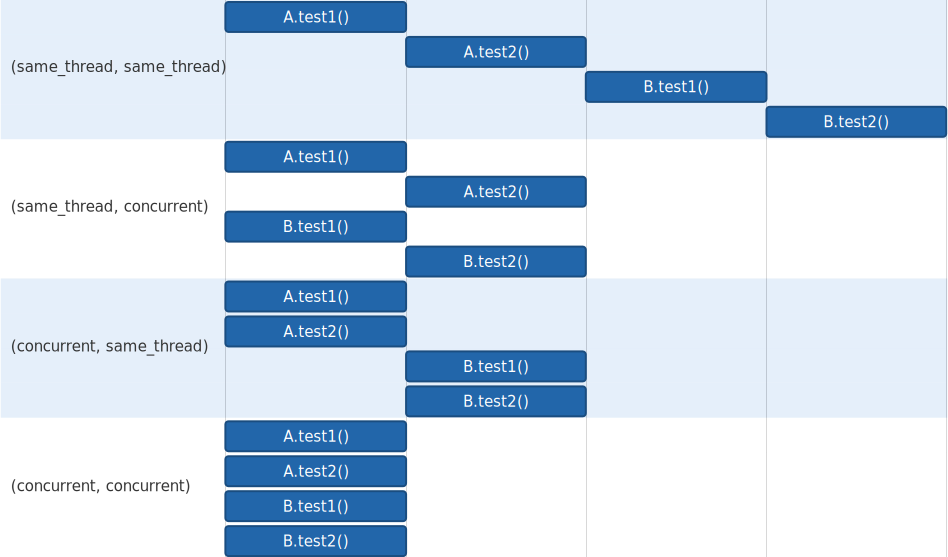
\includegraphics[scale=0.49]{concurrent-test-modes.pdf}}}
      \end{picture}
    \end{frame}

  \section{Fazit}
    \begin{frame}{Fazit}
      \begin{itemize}
        \item Unit-Tests testen Klassen und Methoden
        \item JUnit ermöglicht einfache Unit-Tests in Java
        \item Eclipse unterstützt nativ JUnit 5
        \item Durch fortgeschrittene Funktionalitäten skaliert JUnit auch für größere Projekte
        \item Unit-Tests garantieren nicht die Funktionalität der Applikation im Ganzen
      \end{itemize}
    \end{frame}

	\section*{}
    \begin{frame}{Quellen}
      \begin{itemize}
        \item \url{https://junit.org/junit5/}
        \item \url{https://junit.org/junit5/docs/current/user-guide}
        \item
          \url{https://junit.org/junit5/docs/current/user-guide/images/writing-tests_execution_mode.svg}
        \item
          \url{http://kleuker.iui.hs-osnabrueck.de/CSI/Methoden/kombiquAequivalenzklassenanalyse.html}
        \item
          \url{https://www.eclipse.org/community/eclipse_newsletter/2017/october/article5.php}
        \item \url{https://www.agilealliance.org/glossary/tdd/}
      \end{itemize}
    \end{frame}
    \begin{frame}[c]{Folien, Quellcode Live-Demo}
      \Large
      \centering
      \url{https://github.com/sdoering01/junit-presentation}
    \end{frame}
    \begin{frame}[c]
      \Huge
      \centering
      Vielen Dank für Ihre Aufmerksamkeit!

      Haben Sie noch Fragen?
    \end{frame}

\end{document}
